% Mathematical decomposition tree using three-point linear extrapolation.
\documentclass[border=2pt]{standalone}
\usepackage{tikz}
\usetikzlibrary{trees}

\tikzset{
  term/.style={draw,circle,minimum size=9mm,inner sep=1pt,fill=blue!10},
  leaf/.style={draw,rounded corners=2pt,minimum width=14mm,minimum height=8mm,inner sep=1pt},
  every edge from parent/.style={draw,thick}
}

\begin{document}
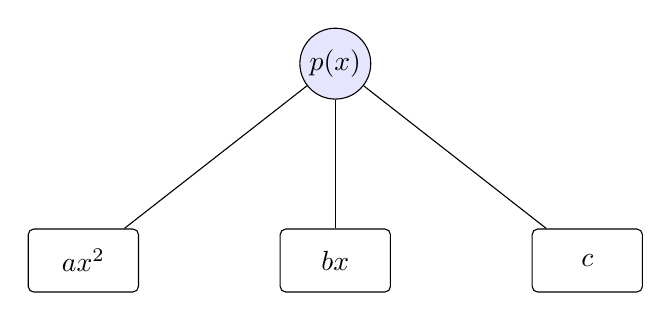
\begin{tikzpicture}[
  grow via three points={one child at (0,-11mm) and
    two children at (-16mm,-18mm) and (16mm,-18mm)}
]
  \node[term] {$p(x)$}
    child {node[leaf] {$ax^2$}}
    child {node[leaf] {$bx$}}
    child {node[leaf] {$c$}};
\end{tikzpicture}
\end{document}
